\documentclass[10pt,a4paper]{article}
\usepackage[utf8]{inputenc}
\usepackage[english]{babel}
\usepackage{graphicx}
\usepackage{lmodern}
\usepackage{kpfonts}
\usepackage[left=2cm,right=2cm,top=2cm,bottom=2cm]{geometry}
\usepackage{algorithm}
\usepackage[noend]{algpseudocode}
\usepackage{wrapfig}
\newtheorem{theorem}{Theorem}
\newtheorem{definition}{Definition}
\newtheorem{notation}{Notation}

\author{Megi Dervishi}
\title{Algorithms and Programation}
\begin{document}
\maketitle
\section*{Homework 1 (09/10/2019)}
\subsection*{Exercise 1}
\subsection*{Solution}
\begin{enumerate}
\item Let $n$ be the size of the array. We will first perform insertion until $\frac{n}{2}$. Then everytime we add a new element the array would expand and if we delete an element the size would cut in half. For example we can have the following sequence of operations which would result in expansion one time and shrinking two times i.e. a very big amortized cost ($\mathcal{O}(n)$)
\begin{center}
Add , Del , Del, Add, Add, Del, Del ...
\end{center}

\item Instead of shrinking by $1/2$ we can shrink by $1/4$ of the size of the array. We can still expand twice the size of the array when inserting an element. This way the deletion cost is "covered" by the insertion.
\end{enumerate}

\subsubsection*{Notations:}

\begin{enumerate}
\item $\Phi _i$ := Potential after the operation $i$ 
\item $c_i$ := Capacity(size) of the array after the operation $i$ 
\item $n_i$ := Number of elements in the array after the operation $i$ 
\item $\alpha_i$ := The Load factor which is the faction of the number of elements stored in the array over the capacity(size) after operation $i$\\
\end{enumerate}
\subsubsection*{Definitions:}

We define the potential as:
$$
\Phi_i := \begin{cases}
2 \cdot n_i - c_i    \quad\text{ if }  \alpha_i \geq \frac{1}{2}\\
\frac{c_i}{2} - n_i  \quad  \text{ if } \alpha_i < \frac{1}{2}
\end{cases}
$$
where $\Phi_0 = 0$, $\Phi_i = 0$ when $\alpha_i = \frac{n_i}{c_i}= \frac{1}{2}$, $\Phi_i = n_i$ when $\alpha_i = \frac{1}{4}$ and $\Phi_i \geq 0 ,\, \forall i \geq 0$.\\

\subsubsection*{Proof}
There are two operations which have their own specific cases depending on the load factor at position $i$ and $i-1$: Insertion and Deletion of an element.\\


\textbf{Insertion}\\
Insertion has the following definition $n_i = n_{i-1} + 1 \quad \quad \quad \quad (\star)$
\begin{itemize}
\item case 1: $\alpha_{i-1} \geq \frac{1}{2}$ \\
(proof from lecture, constant amortized cost $\mathcal{O}(1))$
\item case 2: $\alpha_{i} < \frac{1}{2} \land \alpha_{i-1} < \frac{1}{2} $\\
Since load factor is smaller than half then there is no expansion i.e. $c_i = c_{i-1}$ Using $(\star)$ we obtain:
$$
\hat{t}_i = t_i + \Phi_i -\Phi_{i-1}
= 1 + (\frac{c_i}{2} - n_i) - (\frac{c_{i-1}}{2} - n_{i-1})
$$
$$
=1 + (\frac{c_i}{2} - n_i) - (\frac{c_{i}}{2} - (n_{i} - 1)) = 0 \leq \mathcal{O}(1)
$$

\item case 3: $\alpha_i \geq \frac{1}{2} \land \alpha_{i-1} < \frac{1}{2}$\\
Expansions may not occur here either and $c_i / 2 = n_i$ so we have:
$$
\hat{t}_i = t_i + \Phi_i -\Phi_{i-1}
= 1 + (\frac{c_i}{2} - n_i) - (2n_{i-1} - c_{i-1})
$$
$$
= 3 + 3\frac{c_i}{2} - 3n_i = 3 + 3\frac{c_i}{2} - 3\frac{c_i}{2}
= 3 \leq \mathcal{O}(1)
$$
So for all cases the amortized cost is constant.
\end{itemize}

\textbf{Deletion}\\
Deletion has the following definition $n_i = n_{i-1} - 1 \quad \quad \quad \quad (\spadesuit)$
\begin{itemize}
\item case 1 : $\alpha_i \geq \frac{1}{2} \land \alpha_{i-1} > \frac{1}{2}$
\\Here shrinking may not happen as the load factor is bigger than half i.e. $c_i = c_{i-1}$. Using $(\spadesuit)$ we get:
$$
\hat{t}_i = t_i + \Phi_i -\Phi_{i-1}
= 1 + (2n_{i} - c_{i}) - (2n_{i-1} - c_{i-1}) = -1 = \mathcal{O}(1)
$$
\item case 2: $\alpha_i < \frac{1}{2} \land \alpha_{i-1} = \frac{1}{2}$
Shrinking does not occur. 
$$
\hat{t}_i = t_i + \Phi_i -\Phi_{i-1}
= 1 + (\frac{c_i}{2} - n_i) - (2\frac{1}{2} -1)  
$$
$$
= 1 + (\frac{c_i}{2} - n_i) = 1 + (n_i+1 - n_i) = 2 =\mathcal{O}(1)
$$
\item case 3: $\alpha_{i-1} = \frac{1}{4}$
\\Shrinking happens so the capacity and the number of elements halfs and also we observe that $t_i = n_i +1$
$$ 
\hat{t}_i = t_i + \Phi_i -\Phi_{i-1} = 
n_i +1 + (\frac{c_i}{2} - n_i) - (\frac{c_{i-1}}{2}-n_{i-1})
$$
$$
= n_i + 1 - n_i = 1 = \mathcal{O}(1)
$$
\item case 4: $\frac{1}{4} \leq \alpha_i < \frac{1}{2}$
$$ 
\hat{t}_i = t_i + \Phi_i -\Phi_{i-1} = 
1 + (\frac{c_i}{2} - n_i) - (\frac{c_{i-1}}{2}-n_{i-1})= 2 = \mathcal{O}(1)
$$
\end{itemize}
In conclusion we have shown that the amortized cost for this potential (and method) is constant.


\subsection*{Exercise 2}
\subsection*{Solution}

\subsubsection*{(1)} Assuming that we have $f$ such that it computes any value in F in constant time then we would have the following:

\begin{algorithm}
\caption{Distance between two Strings}\label{ed}
\begin{algorithmic}[1]
\Procedure{Edit\_ Distance (S,T)}{}
\State $\textit{n} \gets \text{ length of string } \textit{S}$
\State $\textit{n} \gets \text{length of string } \textit{T}$
\State $\textit{Tab} \gets \text{Table }\text{of size } n \times n$
\For{ all $i \gets 1$ to $n$ by jumping $\textit{t}$}
	\For{ all $j \gets 1$ to l to $n$ by jumping $\textit{t}$}
		\State $B \gets Tab [i][j]$
		\State $A = Tab[i : i+t] [j]$
	     \State $C = Tab[i] [j: j+t]$
	     \State $D = S[ i : i+t]$
	     \State $E = T [ j: j+ t]$
	     \For{ k $\rightarrow$ 1 to $\textit{t}$}
	    		 	\For {l $\rightarrow$ 1 to $\textit{t}$}
	    		 		\State $Tab[i+k][j+l] \gets f(A,B,C,D,E)$
				\EndFor
		\EndFor
	\EndFor
\EndFor
\EndProcedure
\end{algorithmic}
\end{algorithm}

Time Complexity: $\mathcal{O}((\frac{n}{t})^2 \cdot t^2) = \mathcal{O}(n^2)$


\subsubsection*{(2)}
Take $(i,j)$ then it is trivial to see that $|Tab(i - 1, j) - Tab(i, j)| \leq 1$ since moving left (resp. up, right and down) corresponds simply to a single string operation i.e. to go left, right, up or down one requires only one deletion or one insertion. Moving in diagonal corresponds to a replacement, which has a cost of 0 if the two characters of the alphabet are identical and 1 otherwise. So no matter the direction: left, up, right, down, superior left diagonal $\ldots$ each movement corresponds only to 1 string operation of cost lesser or equal to 1. So every cell has at most 1 of difference from its neighbors.

\subsubsection*{(3)}
To compute the value of a cell in $F$ one does $\min(a,b,c)$ where $a,b,c$ are values in $A,B,C$ plus some constant. Then:
$$\min (a-B, b-B, c-B) = \min(a,b,c) -B $$
Therefore
$$f(A - B,0,C-B,D,E)  = f(A,B,C,D,E)- B$$ 
$$f(A' - B',0,C'-B',D',E')  = f(A',B',C',D',E')- B' $$
Since $ A-B = A'-B', \, C-B = C'-B',\, E=E',\, D=D'$ then we have:
$$f(A, B,C,D,E) = f(A',B',C',D',E') - (B' - B)$$

\subsubsection*{(4)}
We saw in the previous question that we can pre-compute $f$ using $B=0$ and calculate values for $B \neq 0$ by simply adding a constant.  From question 2 we know that the distance in between terms is of at most 1. Then at each term of the list we have $A_{i + 1} = A_i + \Bigg|\begin{matrix}
1\\0\\-1
\end{matrix}$. Therefore for each term we have 3 choices, and we have a total of $t$ terms, so from combinations we know that we have $3^t$ possibilities.This means that we have $3^t$ possible lists for $A$ (and $C$), so a total of $3^{2t}$ possible inputs for $A, C$. Now since we assumed the alphabet has a finite constant size we know that by the same reasoning we have $\sigma^{2t}$ possibilities for $D, E$. Then for any given input we need to compute every term of $F$ i.e. $(t-1)^2$ terms. So in total to compute one cell our algorithm would be $\mathcal{O}(3^{2t} \sigma^{2t} (t - 1)^2) =  \mathcal{O}(3^{2t}\sigma^{2t}t^2)$.

\subsubsection*{(5)}
We have to find a way to store the values of $f(A, B, C, D, E)$, since we have $(3\sigma)^{2t}$ possible inputs. An easy way to store them would be in a tree of depth $4t$ where the root is $B$, the first $t$ layers each node would have 3 branches representing the term fact that $A_{i+1} = A_{i} + \Bigg|\begin{matrix}
1\\0\\-1
\end{matrix}$. The layers $t$ to $2t$ would be structured the same and represent the list $C$. Finally in the layers $2t$ to $3t$ nodes would have $\sigma$ branches to construct $D$ and identically layers $3t$ to $4t$ would construct $E$. Since our tree has a depth of $4t$ a lookup in it is of order $\mathcal{O}(t)$. Then we have (we store directly the value from which the root has been removed):
\begin{algorithm}
\caption{Optimized}\label{euclid}
\begin{algorithmic}[1]
\Procedure{Edit\_Distance (S,T)}{}
\State $\textit{n} \gets \text{ length of string } \textit{S}$
\State $\textit{n} \gets \text{length of string } \textit{T}$
\State $\textit{Tab} \gets \text{Table }\text{of size } n \times n$
\For{ all $i \gets 1$ to $n$ by jumping $\textit{t}$}
	\For{ all $j \gets 1$ to l to $n$ by jumping $\textit{t}$}
		\State $B \leftarrow Tab[i, j]$
		\State $A \leftarrow Tab[i, j:j+t] - B$
		\State $C \leftarrow Tab[i:i+t, j] - B$
		\State $D \leftarrow S[i:i+t]$
		\State $E \leftarrow T[j:j+t]$
		\State $Tab[i+1:i+t, j+1:j+t] \leftarrow Lookup\_ f(A, 0, C, D, E) + B$
	\EndFor
\EndFor
\EndProcedure
\end{algorithmic}
\end{algorithm}

The two for loops give complexity $\mathcal{O}(\frac{n^2}{t^2}k)$ where $\mathcal{O}(k)$ is the complexity of the computations inside. Now looking at those more in detail all the setting and manipulations from line 8 to 11 would be linear in $t$ and the complexity of the lookup is also linear in $t$ (as discussed previously), so overall the complexity of the whole algorithm is: $\mathcal{O}(\frac{n^2}{t})$. Since we are free on the value of $t$ we can choose $t = \log n$ and we get an algorithm that runs in $\mathcal{O}(\frac{n^2}{\log n})$. While in memory it costs $\mathcal{O}((3\sigma)^{2\log n})$ so in total it would take $\mathcal{O}(n^2 + (3\sigma)^{2\log n}) = \mathcal{O}(n^2 + \exp(2\log (3\sigma)\log n)) = \mathcal{O}(n^2 + n^{2\log(3\sigma)})$.

\subsection*{Exercise 3}
\subsection*{Solution}
\begin{center}
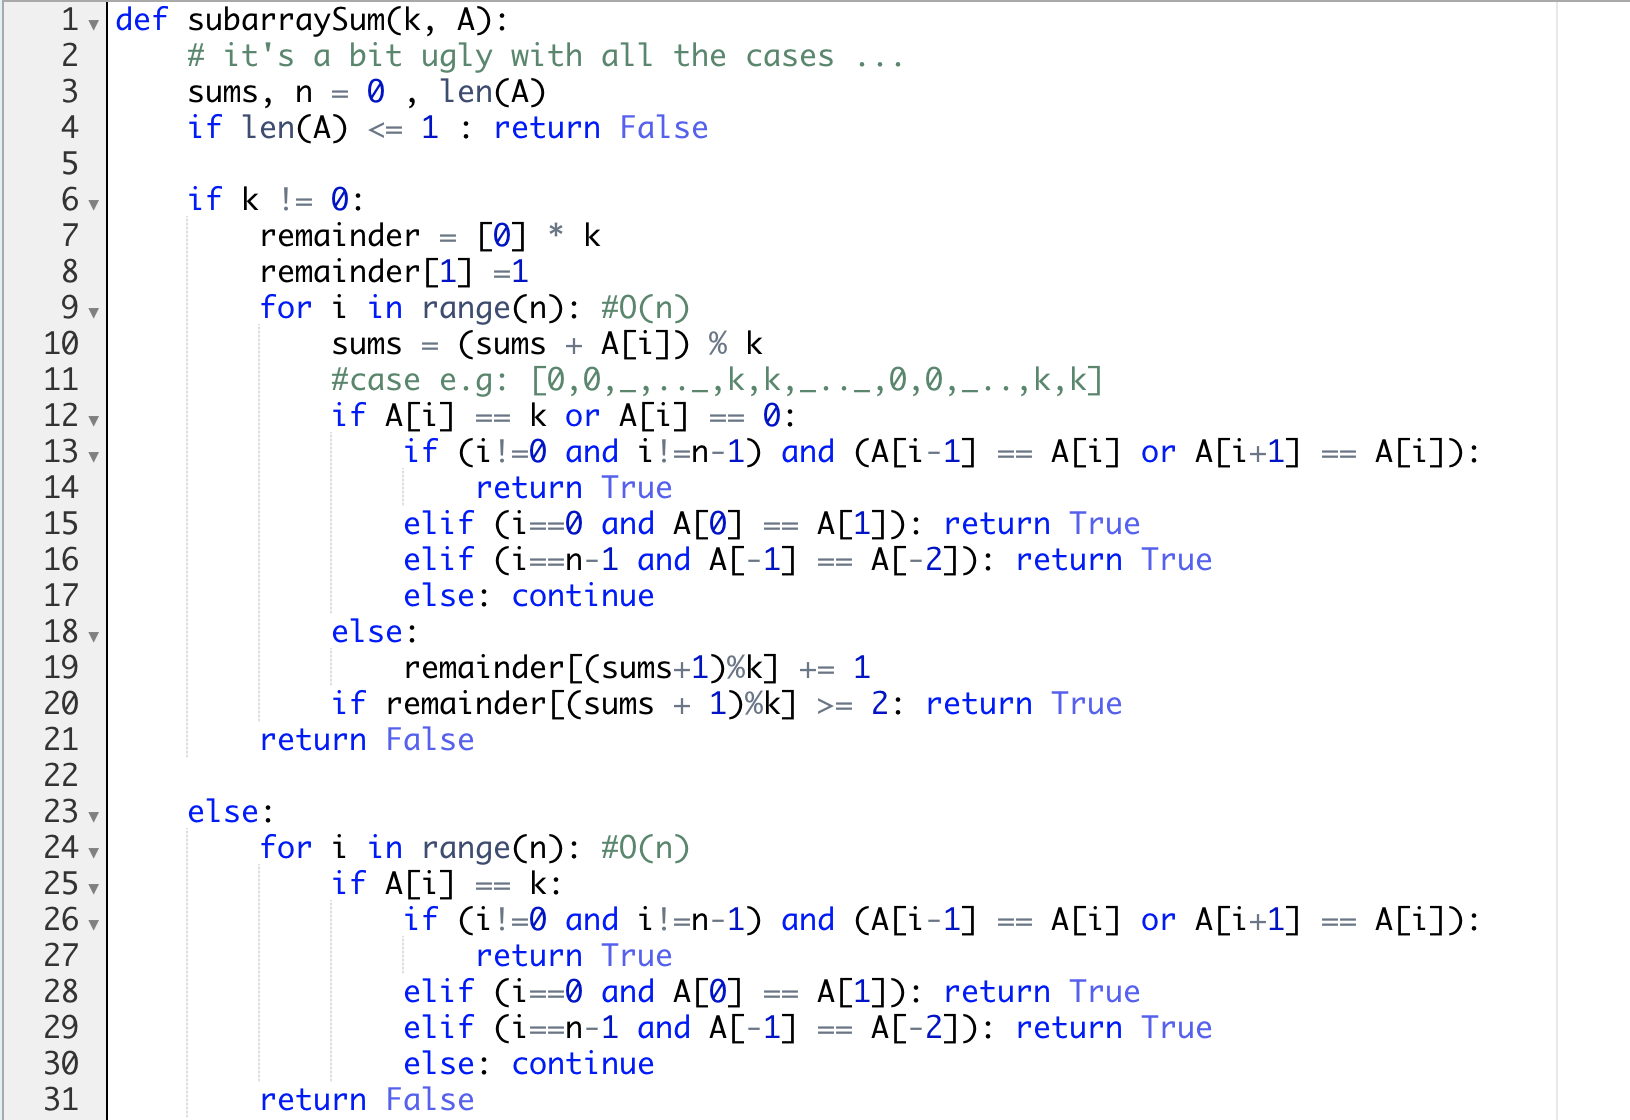
\includegraphics[width=\textwidth]{subarray}
\end{center}
\subsection*{Exercise 4}
\subsection*{Solution}
\begin{center}
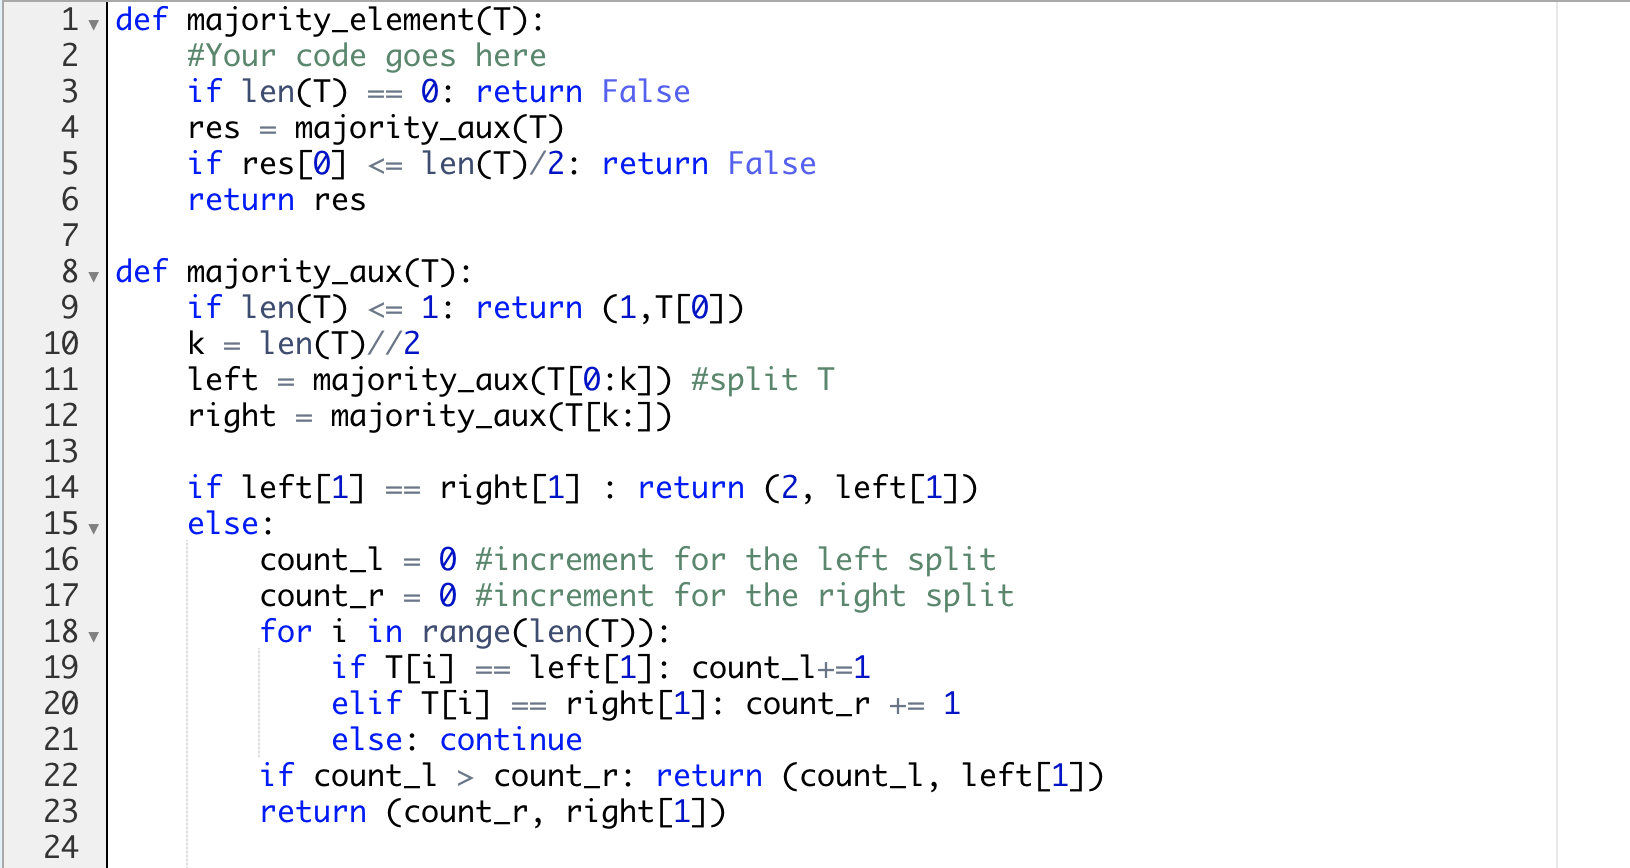
\includegraphics[width=\textwidth]{majority}
\end{center}
\subsection*{Exercise 5}
\subsection*{Solution}
\begin{center}
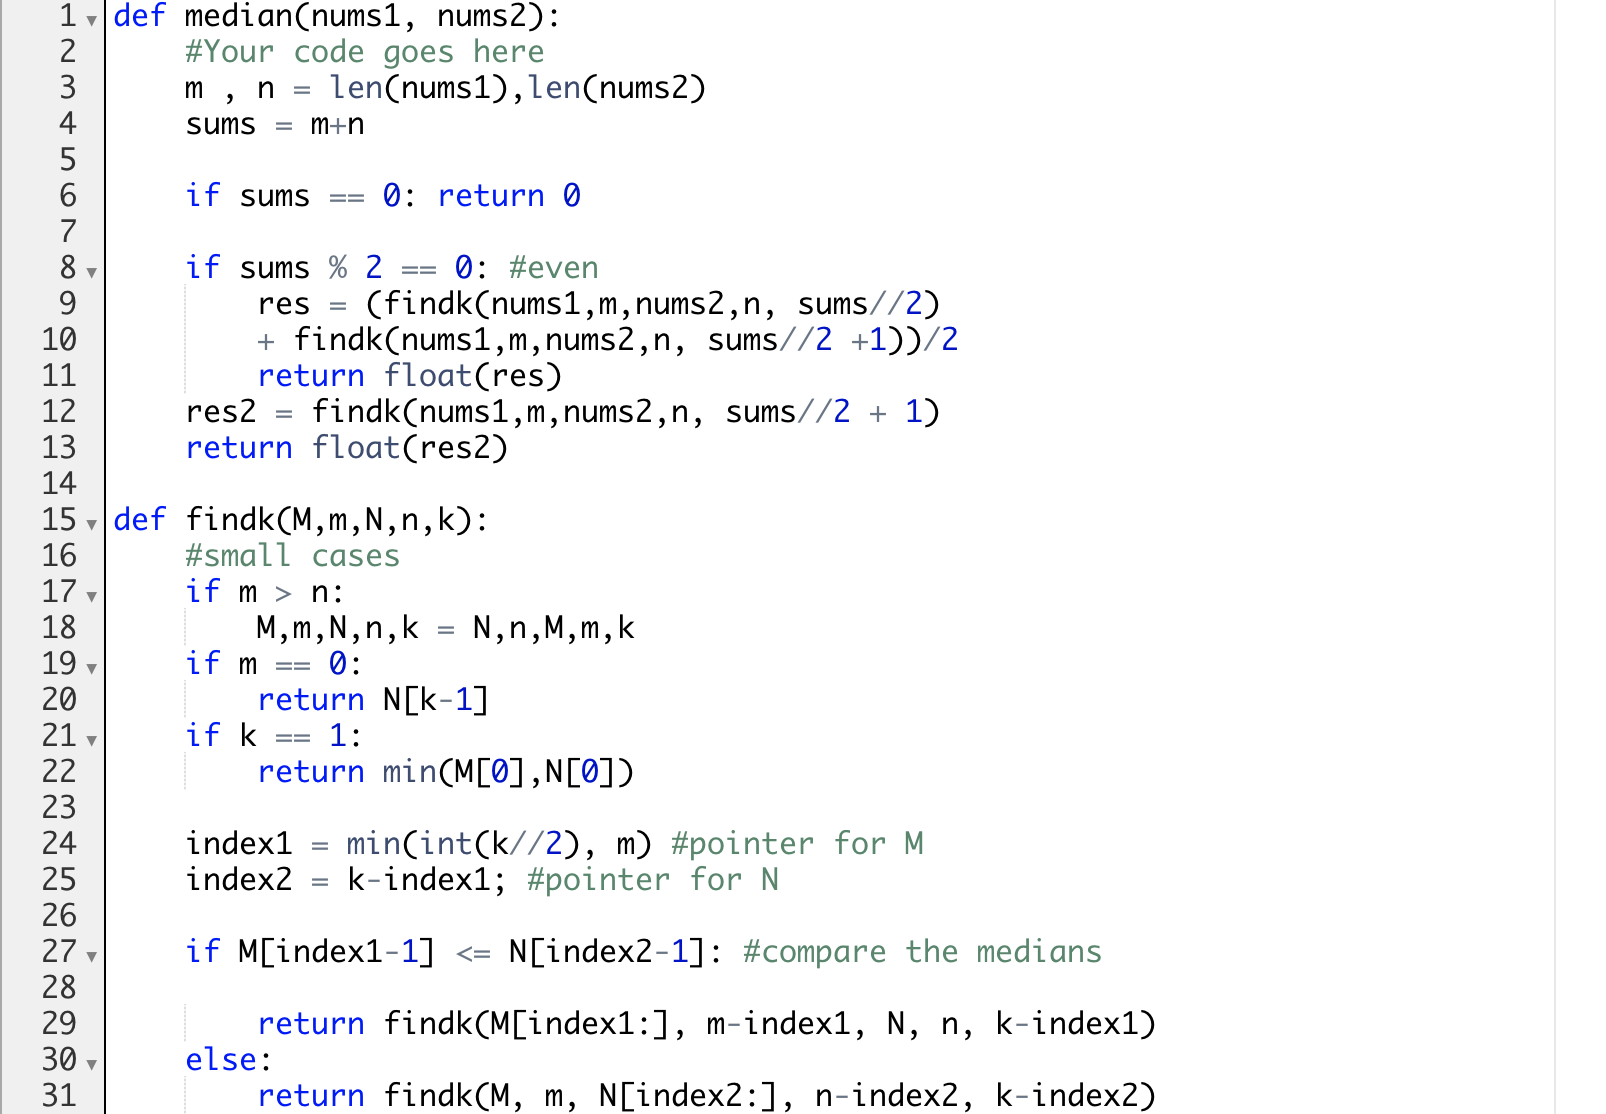
\includegraphics[width=\textwidth]{median}
\end{center}
\break

\break
\section*{Appendix A (Questions)}
\subsection*{Exercise 1.1}
We have seen how dynamic arrays enable arrays to grow while still achieving constant-time amortized performance. This problem concerns extending dynamic arrays to let them both grow and shrink on demand.
\begin{enumerate}
\item Consider an underflow strategy that cuts the array size in half whenever the array falls below half full. Give an example sequence of insertions and deletions where this strategy gives a bad amortized cost.
\item 
Then, give a better underflow strategy than that suggested above, one that achieves constant amortized cost per deletion. Prove that the amortized cost is indeed constant.
\end{enumerate}

\subsection*{Exercise 1.2}

\begin{wrapfigure}{r}{0.25\textwidth}
    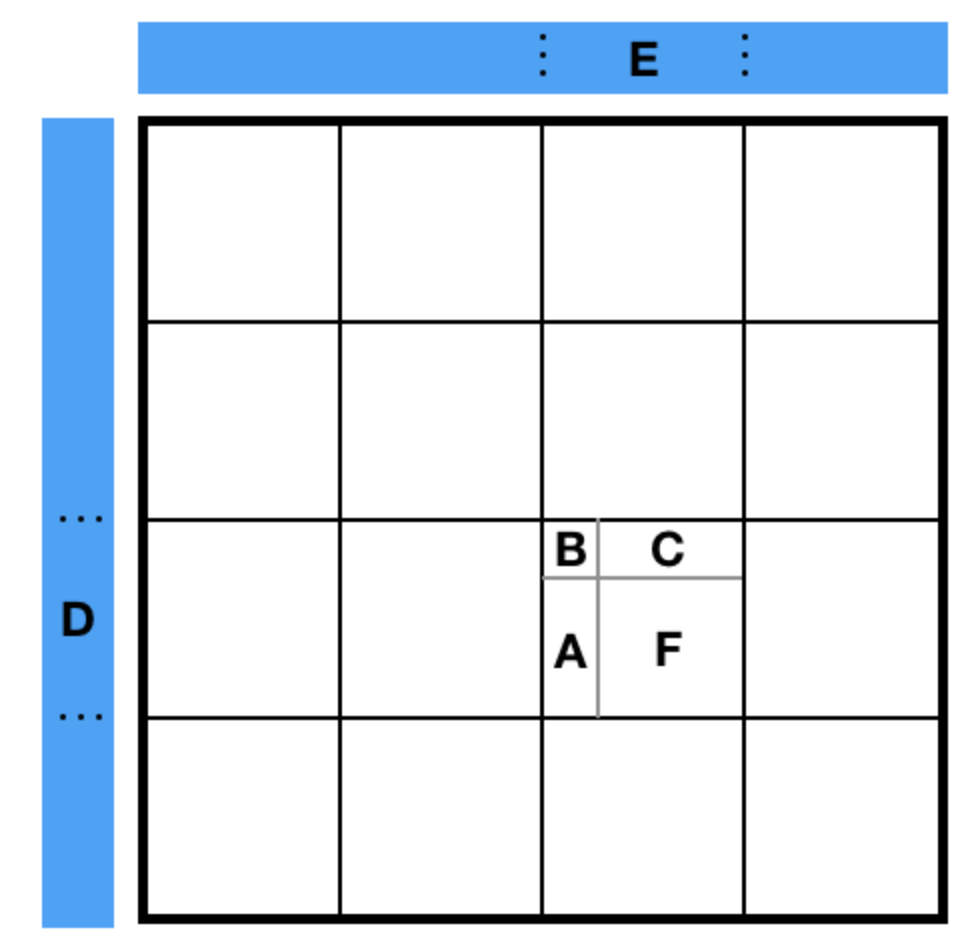
\includegraphics[width=0.25\textwidth]{table}
\end{wrapfigure}
The edit distance between two strings $S,T$ is defined as the minimum number of edit operations that are required in order to transform $S$ to $T$. The edit operations are: substitution (replace one letter of $S$ by another letter), deletion (delete one letter of $S$), or insertion (insert one letter). Your task is to develop a dynamic programming algorithm that computes the edit distance between strings $S$ and $T$, both of length $n$, in O($n^2/\log n$) time. You can assume that the size of the alphabet of $S$ and $T$, $\sigma$ is constant.

Recall the $O(n^2)$-time dynamic programming algorithm for computing the edit distance. Let $D$ be the dynamic programming table. Divide this table into non-overlapping square blocks of size $t \times t$ (see the figure below). Note that the block's values $F$ depend only on the first column $A$, the first row $C$, the corner value $B$, and the substrings $D, E$ of $S,T$, resp.

Suppose that you have a function f that takes $A,B,C,D,E,$ preprocesses them, and after that can compute any value in F in constant time. \begin{enumerate}
\item Modify the dynamic programming algorithm to use the function f.
\item Show that the values in any two neighbouring cells (by side or by corner) differ by at most one.
\item Consider two different blocks corresponding to values A, B,C,D,E and $A',B',C',D',E'$. Suppose that after subtracting $ B$ from every value in $A$ and $C$ and $B'$ from every value in $A'$ and $C'$, we have $A=A',B=B',C=C',D=D',E=E'$. What can you say about the values of the function f for these blocks?
\item Show that you can precompute the values of the function f in $O(3^{2t}\sigma ^{2t}t^2)$ time for all possible $A,B,C,D,E$ simultaneously.
\item Derive an $O(n^2/ \log n)$-time algorithm for computing the edit distance.
\end{enumerate}

\subsection*{Exercise 1.3}
Given a list of non-negative numbers and a target non-negative integer k, write a function subarraySum(k, A) to check if the array has a continuous subarray of size at least $2$ that sums up to a multiple of k, that is, sums up to $p \cdot k$ where p is also an integer. The function must output True if there is such a subarray and False otherwise.

The running time of your algorithm must be $O(n)$. Don't use any data structures excepts for lists.


For example:
\begin{center}
\begin{tabular}{| l | l |}
\hline
Test	 &Result\\
\hline
print(subarraySum($2, [1,2,4,3,5]$)) & True\\
\hline
\end{tabular}
\end{center}


\subsection*{Exercise 1.4}
The majority element of an array is the element that appears  more than  n/2 times (and thus there is at most one such element). Given a list of integers T, develop a recursive algorithm that returns False if T does not contain a majority element, and otherwise returns a tuple of two integers nb, elt where elt is the majority element of T and nb the number of times it appears in T.


For example:
 \begin{center}
\begin{tabular}{| l | l |}
\hline
Test	& Result\\
\hline
print(majority\_ element([1, 1, 100, 7, 100, 100, 7, 100, 100])) & (5, 100)\\
\hline
print(majority\_ element([1,2,1,2])) & False\\
\hline
\end{tabular}
\end{center}
 
\subsection*{Exercise 1.5}
Let $T$ be a sorted array. The median of $T$ is its $(k+1)$-th element if $T$ is of length $2k+1$, and the average of its $k$-th and $(k+1)$-th elements if it is of length $2k$. Let $T_1$ and $T_2$ be two sorted arrays. The median of $T_1$  and $T_2$ is the median of the array obtained by merging $T_1$ and $T_2$. 

Let $nums1$ and $nums2$ be two sorted array of size m and n respectively. Write a function $median(nums1,nums2)$ that finds the median of $nums1$ an $nums2$. The algorithm must run in time complexity $O(\log (m+n))$ (in particular you have no time to merge the two arrays).

You may assume $nums1$ and $nums2$ cannot be both empty.

DO NOT CHANGE THE NAME OF THE FUNCTION.

For example:
\begin{center}
\begin{tabular}{| l | l |}
\hline
Test	 &Result\\
\hline
print(median([2,5,9,14],[3,7,8,12]))& 7.5\\
\hline
\end{tabular}
\end{center}



\end{document}